\section{A Model of Chokepoint Bargaining}\label{sec:model}

The model has three players: Europe ($E$), the United States ($U$) and China ($C$). Europe decides whether ASML's most advanced tools, and the engineers who keep them running, reach Chinese fabs. We treat Europe as one actor; \cref{sec:decide} in the supplement separates the Dutch licensing authority, the firm and the European Union, and \cref{app:notation} collects the notation.

\subsection{Setup}\label{sec:setup}

\paragraph{Alignment and stakes.} Europe chooses an alignment $a\in\{A,X\}$. Under Atlantic alignment ($A$) ASML complies with US denial requirements. Exit ($X$) is a broad realignment of the chokepoint: Europe lets ASML sell and service EUV and advanced immersion DUV tools for Chinese fabs against US objection. China gains $W>0$ from exit, of which a share $\theta\in[0,1]$ can be blocked by US jurisdiction over China-bound flows (the foreign direct product rule, de minimis rules and controls on US-made subsystems). That jurisdiction leaves ASML's supply to US-aligned fabs untouched, so we treat it as credible. The United States loses $V>0$ if Europe exits: $V$ is the patron's dependence on the chokepoint, what it gives up in the AI race when Chinese fabs gain the share $1-\theta$ of access that flow jurisdiction does not block.

\paragraph{Instruments and the baseline.} Washington's instruments $j$ are the core defence guarantee, force posture and enablers, access to frontier AI, and ASML's access to US inputs, persons and customers. After Europe chooses $a$, the United States sets each at a level $x_j(a)$ that is sequentially rational given its commitments, and Europe values it at $v_j(x_j)$. The conditional part of instrument $j$ is $d_j=v_j(x_j(A))-v_j(x_j(X))\ge 0$. The baseline is $x_j(A)$, Washington's ex post optimal provision to a loyal ally. A transfer is a promised increment above this baseline, and a threat is a withdrawal below it, so each instrument is counted once.

\paragraph{Commitment.}\label{sec:commitment} One commitment technology governs every promise and every threat. Before Europe moves, each great power $i$ may attach a stake $m\le\bar m_i$ to any public conditional commitment, which it forfeits if the condition is met and it does not act. The stake is a reduced form for the audience costs of backing down, which tie hands rather than sink costs \citep{fearon1994domestic, fearon1997signaling}, and the cap applies to each commitment separately. A promise to pay $\tau$ after Europe has moved is honoured if and only if $\tau\le\bar m_i$, and a threat whose execution costs the threatener $e$ ex post is credible if and only if $e\le\bar m_i$. Creating a stake costs nothing, and a threat that deters is never carried out. Every withdrawal from a loyal Europe has $e\ge 0$, because the baseline is Washington's ex post optimum.

\subsection{The exit premium}\label{sec:security}

\paragraph{Conditional parts.} In a crisis, Washington defends Europe if its net stake exceeds a crisis-specific cost $\xi$ drawn from a continuous distribution $G$. Its stake in defending a realigned Europe is $s_X=s_0+s_B$, its own interest in European security plus the value of European territory and bases; its stake in a loyal Europe is $s_A=s_X+s_L$; and after exit, defending Europe also forfeits any stake $m_S\le\bar m_U$ on a public threat of abandonment. The conditionality of the core guarantee is
\begin{equation}\label{eq:kappa}
\kappa=G(s_A)-G(s_X-m_S),
\end{equation}
at most $\bar\kappa$ at $m_S=\bar m_U$, and its conditional part is $\kappa S_k$, with $S_k$ Europe's crisis-weighted stake in core defence. Posture and enablers, which can be withdrawn from one ally at a time, have conditional part $d_p$. The AI instrument has conditional part $d_{ai}$; scarce compute makes it cheap to cut an exiter's allocation, and the rescission of the AI Diffusion Rule before its compliance date (\cref{sec:background}) suggests to us that tiering loyal allies is costly, so $d_{ai}$ stays positive. Penalties on ASML itself cost Europe $f$ but also harm US fabs: Washington's ex post gain from penalizing an exiting ASML is $\gamma-c_fV$, so the threat is credible only if $c_fV\le\gamma+\bar m_U$, and its conditional part is $d_f=\chi_ff$ with $\chi_f=\mathbf 1\{c_fV\le\gamma+\bar m_U\}$. As in \citet{wolford2017alliances}, threats against a valuable ally lack credibility, here only for penalties on the firm.

\paragraph{China's offer.} China can promise Europe market access, credit, co-production or relief from its own export controls if Europe exits. A promise of $\tau_C$ costs China $\tau_C$, Europe values it at $\lambda_C\tau_C$ with $\lambda_C\in(0,1]$, and China's promises are capped at $\bar m_C$. With a relative-gains weight $\rho\ge 0$ on Washington's loss, the most China would pay for exit is $W_C=(1-\theta)W+\rho V$, and its credible offer, in units of European utility, is
\begin{equation}\label{eq:omega}
\omega=\lambda_C\min\{W_C,\bar m_C\}.
\end{equation}
If the race is close to zero-sum, $\rho V$ is large and the cap binds, and $\omega$ is set by how far Europe trusts and values Chinese promises. China's observed coercion targets specific acts, such as the 2025 Nexperia export ban after a Dutch order (\cref{sec:record}); we found no case in which China punished a holder for aligning its controls with Washington. We therefore set China's punishment of alignment to zero and treat Chinese coercion as counter-threats attached to particular concessions (\cref{prop:counter}).

\begin{definition}[Exit premium]\label{def:Q}
Exit costs Europe $c=\kappa S_k+d_p+d_{ai}+d_f+\eta$, where $\eta\ge 0$ is the value Europe places on keeping frontier capabilities from a rival that supports Russia's war. Europe's exit premium is China's credible offer net of this credible cost of exit,
\begin{equation}\label{eq:Q}
Q=\omega-c=\lambda_C\min\{(1-\theta)W+\rho V,\ \bar m_C\}-\kappa S_k-d_p-d_{ai}-\chi_f f-\eta .
\end{equation}
Europe's slack is $\Lambda=\pos{-Q}$.
\end{definition}

The premium follows \citet{hirschman1945national}, for whom a state's influence over a partner depends on what the partner would lose by leaving, and slack is the shortfall in Europe's participation constraint in the sense of \citet{clayton2026putting}. \Cref{fig:timing} shows one period: the great powers announce staked promises and threats, bid for Europe's alignment, and Europe chooses; Washington may then issue demands backed by its instruments (\cref{sec:slack}); finally threats are carried out only where that is sequentially rational.

\begin{figure}[t]
\centering
\begin{tikzpicture}[x=1cm,y=1cm,font=\small]
\draw[-{Latex[length=2mm]}, line width=0.6pt, gray] (0,0) -- (14.2,0);
\foreach \x/\lab/\who in {0.8/{US offers $\tau_U\in[0,B_U]$}/{(1)}, 4.4/{China offers $\tau_C\in[0,B_C]$}/{(2)}, 8.0/{Europe chooses $A$ or $X$}/{(3)}, 11.6/{Instruments used}/{(4)}}{
  \fill[black] (\x,0) circle (2pt);
  \node[above=4pt, align=center, text width=3.1cm] at (\x,0) {\who\\ \lab};
}
\node[below=6pt, align=left, text width=5.2cm, font=\footnotesize] at (12.3,0) {US: defend in a crisis?\\ deny frontier AI? penalize ASML?\\ China: restrict critical inputs?};
\end{tikzpicture}
\caption{Timing of the static game. Each instrument in stage (4) is used only if doing so is sequentially rational (\cref{lem:credible}).}
\label{fig:timing}
\end{figure}


\subsection{The price of alignment}\label{sec:bidding}

In the benchmark, Washington and Beijing bid for Europe's alignment in an ascending auction.

\begin{lemma}[Bidding benchmark]\label{lem:bidding}
Suppose the United States and China bid for Europe's alignment in an ascending (clock) auction in which bids are staked promises, Europe values China's promise $\tau_C$ at $\lambda_C\tau_C$, Europe chooses its alignment after the auction, and instruments are then used. Let $\bar z_U=\min\{V,\bar m_U\}$ and $Q=\lambda_C\min\{W_C,\bar m_C\}-c$.
\begin{enumerate}[label=(\roman*)]
\item After alignment $a$, the United States provides $x_j(a)$ for every instrument $j$, so exit lowers Europe's payoff, before transfers, by $c=\sum_j d_j+\eta$.
\item A promise of $\tau$ by power $i$ is honoured if and only if $\tau\le\bar m_i$. Bidding up to one's maximal credible bid (in units of Europe's payoff, $\bar z_U$ for the United States and $Q$ for China) is weakly dominant. In weakly undominated strategies, with an indifferent Europe aligning:
 \begin{enumerate}[label=(\alph*)]
 \item if $Q<V$ and $Q\le\bar m_U$, Europe aligns and the United States pays $\pos{Q}$;
 \item if $Q>\min\{V,\bar m_U\}$, Europe exits, and China's promise gives Europe $\min\{V,\bar m_U\}$ net of $c$.
 \end{enumerate}
 In both cases Europe's payoff is $\pos{\min\{Q,V,\bar m_U\}}$.
\item If $\bar m_U<Q<V$, every binding transfer $\tau\in[Q,V)$ from the United States to Europe would make both Europe and the United States strictly better off than the equilibrium (inefficient exit from limited US commitment).
\end{enumerate}
\end{lemma}

The losing bidder sets the price, a known result (\cref{sec:literature}) that \citet[Supplement B.2]{clayton2026framework} derive for two hegemons. What the lemma adds is the content of $Q$: China's bid enters Europe's participation constraint, and every cost of exit in $c$ is a conditional part that survives sequential rationality. In an alternating-raise auction, subgame perfection alone does not pin down the price if China is indifferent to what Washington pays (\cref{app:proofs}). A rival that values the patron's losses is not.

\begin{remark}[Price driving]\label{rem:spite}
In the alternating-raise auction, let China's relative-gains weight apply to every loss of Washington's, so that China gains $\rho p$ when Europe aligns at price $p$, with $\rho>0$. Let China bid up to its credibility bound $\bar b_C=\lambda_C\bar m_C-c\ge Q$, even where a winning bid would be unprofitable, and let $\bar b_C<\bar z_U-\varepsilon$. Then in every subgame-perfect equilibrium Europe aligns and the price is within $\varepsilon$ of $\pos{\bar b_C}$. If China's cap binds ($W_C\ge\bar m_C$), then $\bar b_C=Q$.
\end{remark}

China raises any bid that Washington will top, since it gains from what Washington pays and never has to honour a bid it does not win. The price is then pinned at China's credibility bound rather than at its willingness to pay. The two coincide when China's cap binds; otherwise what sets the price is how far Europe trusts China's promises, not what exit is worth to China.

\subsection{Agenda power and rupture risk}\label{sec:master}

We now give Europe a voice in the price. Europe and Washington bargain over a perpetual signed transfer flow $P$, with China's credible offer, and hence $Q$, open to Europe as an exit option throughout; $P<0$ means Europe concedes. Agreements bind while Europe's premium stays at $Q$.\footnote{They are enforced by the stake technology; we assume that Washington's cap covers the agreed transfer ($\bar m_U\ge V$ suffices) and that a European concession is a policy Europe would have to reverse publicly. If the premium moves, the two bargain again. A commitment by Europe that survives a change in its premium is what \cref{sec:control} prices.} Every $\Delta$ units of time, Europe proposes with probability $\beta\in[0,1)$ and Washington otherwise. After rejecting a US offer, Europe may exit, which yields flows $Q$ to Europe and $-V$ to Washington forever. If it does not, the dispute ruptures with probability $1-e^{-\lambda\Delta}$; otherwise the status quo continues with flows $(0,0)$, and both discount at rate $r\ge 0$. Rupture is realignment that neither government chooses, for instance after a change of government in The Hague or an unintended escalation: a threat that leaves something to chance \citep{schelling1960strategy}. A rupture puts the parties in the exit state until it is repaired, at rate $\phi\ge 0$, after which bargaining resumes; a chosen exit is permanent.

\begin{proposition}[Bargaining with an outside option and rupture risk]\label{prop:master}
Let $Q<V$, $\beta\in[0,1)$, $r,\lambda,\phi\ge 0$, $r+\lambda>0$, and $r>0$ if $\phi>0$.
\begin{enumerate}[label=(\roman*)]
\item For every $\Delta>0$, every subgame-perfect equilibrium gives Europe the same payoff $x^*(\Delta)$ and the United States $-x^*(\Delta)$.
\item If $\lambda>0$, the subgame-perfect equilibrium is unique (up to Europe's exit choice at one point of indifference, which does not affect payoffs), and agreement is immediate. If $\lambda=0$, there are also stationary equilibria with delay, with the same payoffs.
\item As $\Delta\to 0$, $x^*(\Delta)$ and the equilibrium offer and demand converge to
\begin{equation}\label{eq:master}
P^*=\max\big\{Q,\ \psi\big(Q+\beta(V-Q)\big)\big\},\qquad \psi=\frac{\lambda}{\lambda+r+\phi}\in[0,1].
\end{equation}
If $r+\phi>0$, the second term is the larger one if and only if $Q<\hat Q\equiv\lambda\beta V/(r+\phi+\lambda\beta)$.
\end{enumerate}
\end{proposition}

\begin{figure}[t]
\centering
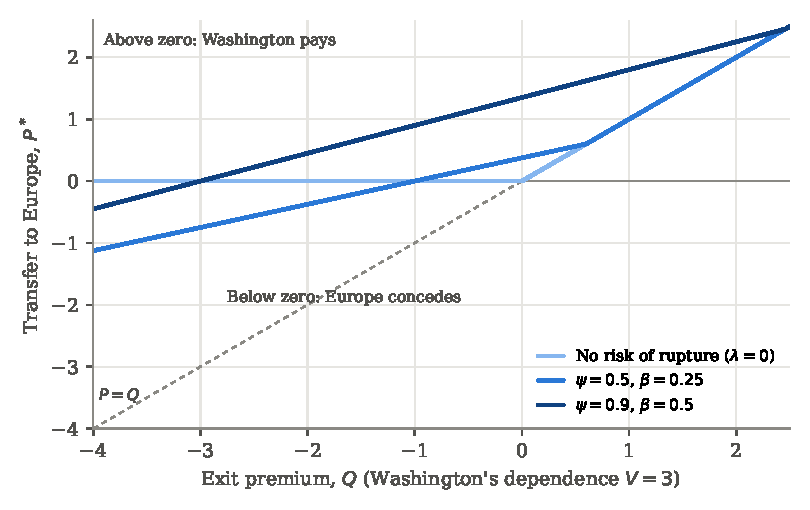
\includegraphics[width=0.75\textwidth]{figures/fig_master.pdf}
\caption{Equilibrium transfer to Europe under rupture risk (\cref{prop:master}) as a function of the exit premium, with $V=3$. Without rupture risk ($\lambda=0$) the transfer is $\pos{Q}$. With rupture weight $\psi=0.5$ and $\beta=0.25$, Washington pays Europe whenever $Q>-1$; with $\psi=0.9$ and $\beta=0.5$, whenever $Q>-3$. Below those values Europe concedes. Every curve lies on or above the dashed line $P=Q$.}
\label{fig:master}
\end{figure}

\begin{corollary}[Threshold and channels]\label{cor:master}
Under the conditions of \cref{prop:master}:
\begin{enumerate}[label=(\alph*)]
\item $P^*\ge Q$: Europe never concedes more than its slack, $-P^*\le\Lambda$.
\item If $\lambda=0$, $P^*=\pos{Q}$; if $\beta=0$, $P^*=\max\{Q,\psi Q\}$. In either case $Q\le 0$ implies $P^*\le 0$.
\item $P^*>0$ if and only if $Q>0$, or $\lambda>0$ and $Q+\beta(V-Q)>0$.
\item Holding $Q$ fixed, $\partial P^*/\partial V=\beta\psi$ where the second term binds ($Q<\hat Q$) and $0$ where $Q>\hat Q$.
\item $V$ enters $P^*$ directly only through the term $\beta\psi V$ (agenda power under rupture risk), and indirectly only through $Q$: through the rival's valuation ($\rho V$ in $W_C$ when the cap does not bind), self-harming sanctions ($\chi_f$ falls to zero as $V$ rises past $(\gamma+\bar m_U)/c_f$) and the silicon shield (if $s_B$ rises with $V$, $\kappa$ moves with a sign that depends on $G$). \Cref{prop:pain} adds a fifth channel, hold-up, which works through Washington's own need for ASML's servicing.
\end{enumerate}
\end{corollary}

The threshold in part (b) is the outside-option principle, and its substance is \citeauthor{wagner1988economic}'s (\cref{sec:literature}). Without rupture risk, a holder whose exit premium is negative gets nothing for its chokepoint, whoever proposes and however much its patron needs it: its only threat is exit, and exit is credible only when $Q>0$. When $\lambda>0$, a rejected demand risks a rupture that costs Washington $V$, so Europe's demands carry weight in proportion to $\beta\psi$, a binary instance of the identity-dependent externalities through which a seller extracts surplus from parties that do not buy \citep{jehiel1996how}. Repair changes only the weight: as $r\to 0$, $\psi$ tends to $\lambda/(\lambda+\phi)$, the long-run share of time that a relationship subject to these shocks spends broken. If ruptures are quickly undone, as when a new government in The Hague would realign and its successor return, Washington's dependence counts only in proportion to how long a rupture would last. The corner $\beta\to 1$, $\lambda\to\infty$, $\phi=0$, in which Europe obtains all of $V$, is the bargaining implied when the summary of \citet{juijn2026europe} calls ASML ``the only card Europe still holds'' (\cref{sec:intro}). It requires take-it-or-leave-it demands whose rejection ends in lasting realignment with near certainty, a commitment Europe has not shown it can make.

Hold-up is the other route by which Washington's need for ASML can raise Europe's price. If disagreement carries flow costs $c_E$ to Europe and $c_U$ to Washington, as when Europe interrupts the servicing of US-aligned fabs, Europe's price becomes $\max\{Q,\ \psi(Q+\beta(V-Q))+(1-\psi)(\beta c_U-(1-\beta)c_E)\}$ with constant costs and permanent rupture (\cref{prop:pain}). \Cref{sec:extensions} summarizes when such an interruption is credible.

Rupture risk cuts both ways. When $Q<0$ and $Q+\beta(V-Q)<0$, a rupture would leave Europe worse off than the aligned status quo, and Washington can extract part of the value to Europe of avoiding it, though never more than Europe's slack (\cref{cor:master}(a)). \Cref{sec:slack} shows that Europe's surplus over exit, whatever bargaining produces it, also caps what Washington obtains by any combination of conditional threats.
